\chapter{Diseño de la Arquitectura y del Sistema}
\label{sec:arquitectura}

\begin{abstract}
En este capítulo se detalla y justifica la elección del stack tecnológico, abordando la arquitectura de comunicación mediante WebSockets, el entorno de ejecución asíncrono en Node.js, el renderizado reactivo con React y un sistema de persistencia dual basado en MariaDB y Redis. A continuación, se expone la estrategia de contenedorización con Docker y la política de pruebas automatizadas para garantizar la calidad y portabilidad del sistema.

Por otro lado, se describe  la materialización técnica, el diseño arquitectónico y la infraestructura tecnológica adoptada para dar solución al sistema analizado previamente. Se detalla la estructura estructural global orientada a componentes bajo un modelo cliente-servidor desacoplado, la justificación de los patrones de diseño en cada subsistema, la topología de red para el tiempo real, así como el diseño de la persistencia híbrida y las medidas de seguridad para la transferencia asimétrica de datos.
\end{abstract}

\section{Marco Tecnológico}

\subsection{Arquitectura de comunicación y sincronización}

Dada la naturaleza interactiva de un juego multijugador, la sincronización en tiempo real entre múltiples clientes es un punto crítico dentro del desarrollo de \textit{King and Peasant}. Para este propósito, implementar el motor del juego sobre una arquitectura web tradicional resultaba inviable debido a las limitaciones estructurales del protocolo \textit{HTTP}. El uso de técnicas como el \textit{Long-Polling} (\textit{polling}), donde el cliente interroga constantemente al servidor en busca de actualizaciones, introduciría una sobrecarga significativa en la red debido al envío repetitivo de cabeceras HTTP, generando latencias perceptibles que degradan la experiencia de juego \cite{rfc6202}.

Como alternativa a una API REST, se decidió utilizar el protocolo \textit{WebSocket} como núcleo de las comunicaciones de la partida. Como define el estándar oficial de la IETF \cite{rfc6455}, esta tecnología proporciona un canal de comunicación bidireccional sobre una única conexión TCP persistente. Esto permite el envío de eventos asíncronos (\textit{server-push}) en el mismo instante en el que se modifica el estado, validando las jugadas y actualizando instantáneamente la interfaz de todos los clientes conectados, reduciendo a su vez el coste computacional y garantizando una sincronización  fluida.

\subsection{Tecnologías de \textit{backend} y Ecosistema de Desarrollo}

El alto volumen de conexiones concurrentes que presenta un juego multijugador exige un entorno de ejecución capaz de gestionar con eficiencia el consumo elevado de recursos que se produce al mantener las conexiones abiertas en un estado de sincronización permanente. En el caso de los servidores web tradicionales, el modelo de concurrencia basado en hilos (\textit{thread-per-request}) se ve afectado por el cambio de contexto (\textit{context switching}) \cite{tilkov_node}, provocando un rápido agotamiento de la memoria y cuellos de botella. Por otro lado, la mantenibilidad del código y el uso de lenguajes unificados constituyó un factor determinante a la hora de decantarse por una arquitectura de servidor. 

Por estos motivos, se adoptó \textit{Node.js}. Su arquitectura basada en un bucle de eventos (\textit{Event Loop}) procesa las solicitudes de red de forma asíncrona, evitando bloquear el hilo principal durante la espera de respuestas de la base de datos o de los clientes. Este diseño arquitectónico permite al sistema mantener activas miles de conexiones bidireccionales de manera simultánea con un consumo residual de recursos. Sumado a las ventajas arquitectónicas de emplear un lenguaje isomórfico, la elección de esta pila tecnológica se sustenta fuertemente en la experiencia previa del equipo de desarrollo. Contar con un conocimiento previo de este entorno reduce de forma drástica la curva de aprendizaje, minimiza la sobrecarga cognitiva y supone una ventaja estratégica para agilizar el ciclo de implementación del proyecto.

\subsection{Tecnologías de \textit{frontend} Reactividad de Interfaz}

La implementación de un juego de mesa en un entorno digital multijugador requiere elementos como un tablero interactivo, el cual, en términos de ingeniería, no es más que la proyección visual de una compleja máquina de estados. Sin embargo, se plantea una serie de retos técnicos a la hora de diseñar este componente. 

En primer lugar, la manipulación directa del \textit{Document Object Model} (DOM) para actualizar la interfaz resulta computacionalmente ineficiente. El navegador se ve obligado a recalcular estilos y repintar la pantalla cada vez que se produce una modificación, lo que provoca que la fluidez de la experiencia se vea degradada \cite{mardan_react}. En segundo lugar, abordar una interfaz que cuenta con tableros, mazos, perfiles y salas de espera bajo una arquitectura monolítica dificultaría enormemente su mantenibilidad y fomentaría la duplicación de código. Finalmente, se le suma el riesgo de desincronización de los estados visuales, resultando en validaciones del \textit{backend} que no se reflejan en la información gráfica \cite{banks_react}.  

Como solución a todos estos problemas, la arquitectura del cliente se construyó utilizando \textit{React}, una librería que impone un paradigma de desarrollo declarativo y basado en componentes. En primer lugar, gracias a la implementación de un \textit{Virtual DOM}, la ineficiencia computacional se mitiga. Al recibir un nuevo evento, \textit{React} genera una representación en memoria de la interfaz y la compara con la actual mediante un algoritmo de diferenciación (\textit{diffing}), aplicando al DOM real únicamente las modificaciones estrictamente necesarias. En segundo lugar, su arquitectura modular minimiza el riesgo que supone construir un sistema monolítico, permitiendo dividir la interfaz en unidades lógicas aisladas e independientes, facilitando la encapsulación y garantizando la mantenibilidad a largo plazo del código. Por último, el paradigma declarativo de \textit{React} permite concibir la interfaz matemáticamente como una función del estado subyacente ($UI = f(estado)$) \cite{banks_react}, convirtiendo el tablero en un reflejo exacto de la información de la partida y las reglas dictaminadas por el \textit{backend} \cite{mardan_react}.

\subsection{Gestión de la persistencia de datos}

Dentro de la información gestionada por el ecosistema encontramos requisitos técnicos independientes, lo que implica la necesidad de implementar un enfoque de persistencia adecuado para cada uno de ellos fundamentado en su naturaleza. Por un lado, la información estructural, como pueden ser las credenciales, perfiles de usuario, historial de partidas o la gestión de salas de espera (\textit{lobbies}), exige un almacenamiento persistente y estructurado que garantice las propiedades ACID (Atomicidad, Consistencia, Aislamiento y Durabilidad) \cite{elmasri_db}. Para satisfacer esta necesidad, y tras evaluar alternativas relacionales robustas como \textit{PostgreSQL}, se seleccionó el motor de bases de datos relacional \textit{MariaDB} por su agilidad en consultas y su perfecta integración con el ecosistema de \textit{Node.js}. Este motor se encarga de gestionar de forma centralizada la información de los usuarios y la configuración inicial de las partidas. La interacción con este motor relacional se abstrajo mediante \textit{Prisma ORM}, una decisión que previene vulnerabilidades de inyección SQL y garantiza un tipado estricto entre el esquema de la base de datos y la lógica del \textit{backend}.

Por otro lado, el estado del tablero interactivo se convierte en un dato efímero sometido a un volumen masivo de operaciones de lectura y escritura concurrentes. Hacer uso de una base de datos relacional para registrar las modificaciones generaría un cuello de botella debido a la latencia de entrada/salida (I/O), ralentizando la comunicación. Para mitigar este problema, se implementó \textit{Redis} como almacén de estructuras de datos en memoria (\textit{In-Memory Data Grid}) \cite{carlson_redis}. A diferencia de sistemas de caché simples como \textit{Memcached}, \textit{Redis} soporta el manejo nativo de estructuras de datos complejas, una característica indispensable para modelar el estado de un juego. Hacer uso de la memoria RAM para almacenar el estado dinámico de la partida permite que el servidor valide y comparta el resultado de las jugadas con tiempos de respuesta mucho menores, delegando en \textit{MariaDB} la persistencia del resultado final una vez concluido el encuentro.

\subsection{Contenedorización y automatización de pruebas}

El complejo funcionamiento intrínsico del motor de reglas asimétrico requería mecanismos rigurosos para garantizar la calidad y la estabilidad del software. El mal funcionamiento de las validaciones de estado o de las transiciones de la partida degradaría la experiencia de juego. En respuesta, haciendo uso de los marcos de trabajo \textit{Jest} y \textit{Vitest}, se implementó una batería de pruebas automatizadas que aseguraban el correcto comportamiento del motor de validación ante cualquier escenario \cite{myers_testing}. Dichas herramientas han permitido aislar y testear unitariamente la lógica del \textit{backend} y los componentes del \textit{frontend}.

De forma paralela, la gestión de la infraestructura se apoyó en la tecnología de contenedores \textit{Docker} \cite{turnbull_docker}. El principal problema que se buscó mitigar con esta adopción fue la inconsistencia de entornos al tratarse de un desarrollo colaborativo entre dos personas. Resultaba necesario aislar los servicios para evitar fallos derivados de las diferencias de \textit{hardware} o configuración del sistema operativo. Por este motivo, se estableció una arquitectura de ejecución híbrida. Por un lado, los servicios de bases de datos (\textit{MariaDB} y \textit{Redis}) se ejecutan exclusivamente mediante contenedores, garantizando que el equipo opere siempre sobre versiones idénticas de estos sistemas. Por otro lado, la capa de aplicación (\textit{frontend} y \textit{backend}) se implementó con un modelo flexible que permite su lanzamiento en local para agilizar la iteración de código, o bien su ejecución contenedorizada. A su vez, esta estandarización de los servicios resulta idónea para simplificar y asegurar el futuro despliegue de la plataforma en entornos de producción.

\section{Diseño de la Arquitectura Global}

El diseño de la arquitectura del sistema constituye el núcleo estructural del proyecto. Se basa en un modelo cliente-servidor fuertemente desacoplado pero integrado bajo un mismo flujo de desarrollo. En la Figura \ref{fig:arquitectura} se ilustra el esquema general del sistema y sus flujos de comunicación físicos.

\begin{figure}[H]
    \centering
    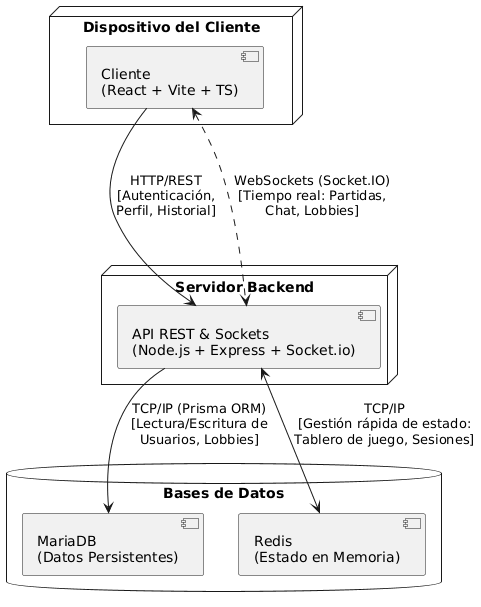
\includegraphics[width=0.7\textwidth]{figures/arquitectura.png}
    \caption{Diagrama de Arquitectura global del sistema y flujos de comunicación.}
    \label{fig:arquitectura}
\end{figure}

\subsection{Estrategia Organizativa: Monorepositorio}
  
En lugar de segregar el cliente y el servidor en repositorios de control de versiones independientes (polirepositorio), se toma la decisión arquitectónica de utilizar un Monorepositorio gestionado de forma nativa mediante \textit{npm workspaces}. 

Esta alternativa se elige principalmente por su capacidad para unificar y simplificar la gestión del ciclo de vida del desarrollo. Al agrupar los módulos de \textit{client} y \textit{server} en un único entorno, se facilita la configuración de la infraestructura local (bases de datos en Docker) y se centraliza la orquestación de comandos. Esto permite que procesos como la instalación de dependencias, la ejecución de pruebas (\textit{testing}) y el despliegue local de toda la pila tecnológica (\textit{frontend}, \textit{backend}, MariaDB y Redis) se realicen con un solo comando desde el directorio raíz, reduciendo la fricción en el entorno de desarrollo y en los flujos de Integración Continua (CI/CD).

\subsection{Arquitectura del Servidor (\textit{backend})}

El servidor se diseña huyendo del patrón de monolito tradicional, apostando por una Arquitectura por Capas estricta. Esta decisión fomenta el principio de responsabilidad única y facilita la creación de pruebas unitarias al aislar el enrutamiento de la lógica funcional. El flujo se divide en:

\begin{enumerate}
    \item \textbf{Capa de Enrutamiento:} Define los \textit{endpoints} HTTP utilizando Express.
    \item \textbf{Capa de Controladores:} Procesa, sanea y valida técnicamente las peticiones.
    \item \textbf{Capa de Servicios:} Encapsula toda la lógica de negocio compleja de forma agnóstica a la red y al transporte.
\end{enumerate}

\paragraph{Paradigma de Comunicación Bidireccional:}
Para el ecosistema de juego, se descartan alternativas arquitectónicas como \textit{Short Polling} o \textit{Server-Sent Events} (SSE). El \textit{Polling} tradicional generaría una sobrecarga HTTP inasumible y latencia en un juego por turnos. Por ello, se justifica el uso exclusivo de WebSockets (\textit{Socket.io}), estableciendo un canal persistente, bidireccional y de muy baja latencia, crítico para sincronizar eventos como el robo de cartas o las notificaciones del chat en milisegundos.

\subsection{Arquitectura del Cliente (\textit{frontend})}

El cliente se modela como una \textit{Single Page Application} (SPA) desarrollada en \textit{React}. En lugar de acoplar la lógica de negocio a la capa de vista, se opta por una arquitectura de componentes funcionales apoyada en Custom Hooks. 

Para la propagación del estado de sesión y de la partida, se descarta el envío manual de propiedades en cascada (\textit{prop drilling}), adoptando el patrón Context API. Esto permite mantener un árbol de componentes limpio y optimizado, donde cada nodo accede únicamente a los datos que necesita, mejorando la mantenibilidad a largo plazo.

\subsection{Arquitectura de Persistencia Híbrida}

Para la persistencia de la información del sistema se diseña un modelo de datos relacional robusto, gestionado a través de \textit{Prisma ORM}. Este modelo soporta la lógica de negocio subyacente, garantizando la integridad referencial y facilitando las consultas complejas. El esquema de la base de datos (\textit{MariaDB}) gravita en torno a cinco entidades principales y sus relaciones, tal y como se ilustra en el diagrama Entidad-Relación de la Figura \ref{fig:modelo_er}.

\begin{figure}[H]
    \centering
    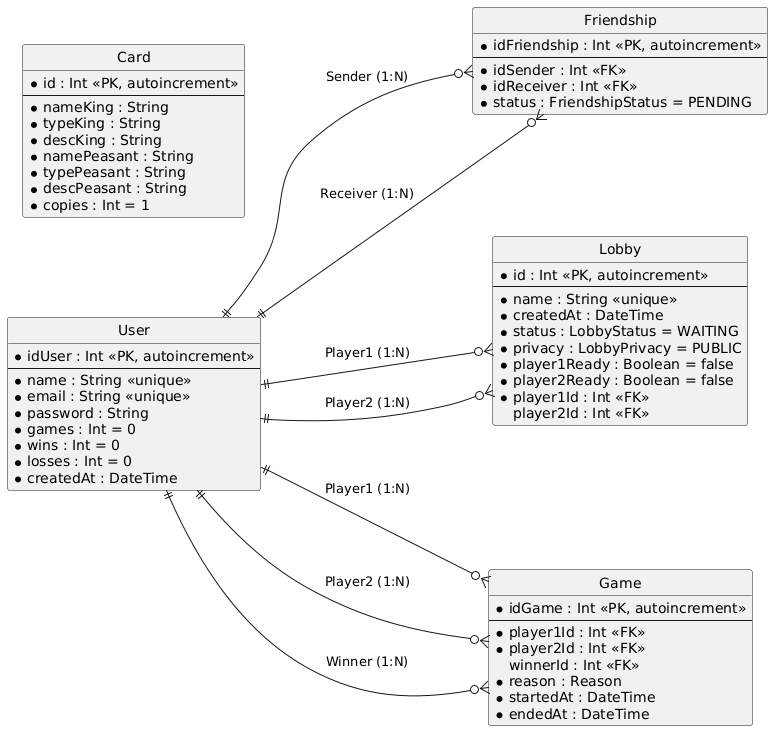
\includegraphics[width=0.9\textwidth]{figures/ER.png}
    \caption{Diagrama Entidad-Relación del sistema.}
    \label{fig:modelo_er}
\end{figure}

\subsubsection{Entidades Relacionales Principales}

\begin{itemize}
    \item \textbf{Usuario (\textit{User}):} Es la entidad central del ecosistema. Además de almacenar las credenciales de acceso (correo y contraseña protegida), centraliza las estadísticas globales del jugador en la plataforma, manteniendo un conteo actualizado de partidas jugadas, victorias y derrotas. Actúa como nodo relacional para el resto de entidades del sistema.
    
    \item \textbf{Amistad (\textit{Friendship}):} Modela la red social del juego. En lugar de utilizar una relación binaria simple de existencia, se diseña con un patrón de estado mediante el enumerado \texttt{FriendshipStatus} (\textit{ACCEPTED, PENDING, DENIED}). Esto permite mantener un control transaccional sobre quién envió la petición (\textit{Sender}) y quién la recibió (\textit{Receiver}), habilitando la gestión asíncrona de invitaciones.
    
    \item \textbf{Sala (\textit{Lobby}):} Aunque la concurrencia y el estado en tiempo real de las salas se delega en la base de datos en memoria (\textit{Redis}) por motivos de latencia, esta entidad define la estructura persistente de la sala. Almacena metadatos críticos como el nivel de privacidad (\textit{PUBLIC/PRIVATE}), el estado actual (\textit{WAITING/ONGOING}) y la confirmación de preparación (\textit{Ready}) de los dos jugadores vinculados.
    
    \item \textbf{Carta (\textit{Card}):} Define los elementos jugables del sistema. Resulta destacable el enfoque de diseño asimétrico aplicado a esta entidad. Para optimizar el esquema y evitar la duplicidad de tablas entre las dos facciones del juego (Rey y Campesino), se opta por un modelo unificado. Cada registro contiene simultáneamente los atributos (nombre, tipo y descripción) de su variante como Rey y su variante como Campesino, centralizando la configuración de los mazos.
    
    \item \textbf{Partida (\textit{Game}):} Constituye el registro histórico del sistema. Relaciona a dos usuarios como oponentes y registra de forma inmutable el identificador del ganador, así como las marcas de tiempo de inicio y fin. 
\end{itemize}

\subsubsection{Estado en Memoria (Redis) y Estructura del \textit{GameState}}

Mientras que \textit{MariaDB} gestiona los datos inmutables y a largo plazo, el núcleo de la partida en vivo reside en \textit{Redis}. El estado del juego (\textit{gameState}) es un objeto JSON complejo que actúa como la única fuente de verdad durante el transcurso de una partida.

Este objeto almacena propiedades persistentes durante el encuentro (como el turno actual, la era, las puntuaciones y los mazos) y atributos volátiles u opcionales que modelan la lógica interna del servidor:
\begin{itemize}
    \item \texttt{pendingAction}: Objeto temporal que pausa el flujo principal de la partida cuando el sistema requiere una decisión asíncrona de un jugador (por ejemplo, seleccionar un objetivo tras jugar una carta de efecto).
    \item Pila de resolución (\texttt{queuedKingMobilize} y \texttt{queuedPeasantDispatch}): Estructuras que permiten encadenar y resolver múltiples acciones secuenciales de forma ordenada.
    \item \texttt{seenByKing}: Bandera booleana (\textit{flag}) introducida por mecánicas específicas de espionaje, que permite asimetría en la visibilidad de una misma carta.
    \item \texttt{lastEvent}: Etiqueta temporal utilizada por el motor interno para procesar condiciones de victoria o cambios de fase, la cual se purga antes de emitir cualquier estado.
\end{itemize}

\subsubsection{Seguridad y Patrón de Transferencia de Datos (DTO)}

Transmitir el \textit{gameState} crudo a los clientes supondría una vulnerabilidad crítica, ya que un jugador podría inspeccionar el tráfico de \textit{WebSockets} mediante las herramientas de desarrollador del navegador y descubrir las cartas ocultas de su oponente.

Para mitigar este riesgo desde el diseño de la arquitectura, se implementa el patrón \textbf{Data Transfer Object (DTO)}. El \textit{backend} nunca expone el estado original de \textit{Redis}. En su lugar, el servicio de juego clona el estado y ejecuta una función de transformación que genera dos vistas asimétricas: \texttt{dtoKing} y \texttt{dtoPeasant} (Figura \ref{fig:dto_pattern}).

\begin{figure}[H]
    \centering
    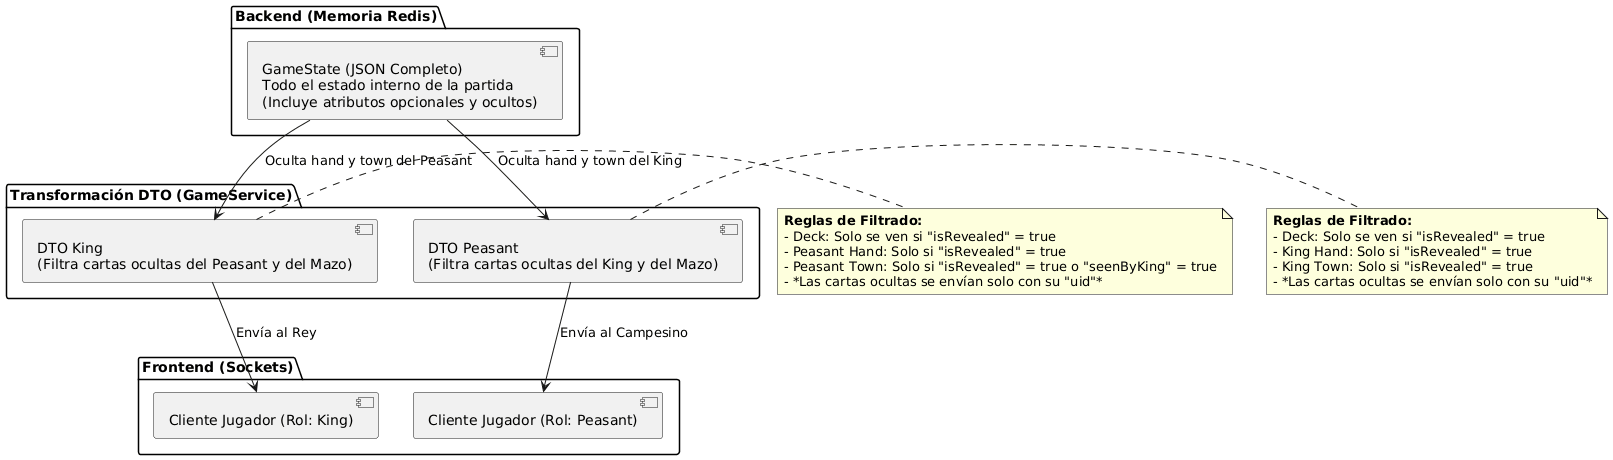
\includegraphics[width=1\textwidth]{figures/dto_flujo.png}
    \caption{Arquitectura de seguridad y filtrado de estado mediante el patrón DTO.}
    \label{fig:dto_pattern}
\end{figure}

Las reglas de filtrado aplicadas por el servidor son estrictas:
\begin{enumerate}
    \item \textbf{Mazo Global (\textit{Deck}):} Cualquier carta no revelada (\texttt{isRevealed: false}) es censurada, transmitiendo al cliente únicamente su identificador único (\texttt{uid}).
    \item \textbf{Censura Asimétrica:} El DTO del Rey recibe la mano y la ciudad del Campesino censurados, a menos que la carta haya sido revelada públicamente o interceptada (\texttt{seenByKing: true}). De forma recíproca, el DTO del Campesino recibe los datos del Rey completamente censurados si no cumplen las condiciones de visibilidad.
\end{enumerate}

Esta capa de transformación garantiza la integridad competitiva del sistema, asegurando que el cliente de React solo procese y renderice la información a la que tiene acceso legítimo.
